\documentclass{template/openetcs_report}
% Use the option "nocc" if the document is not licensed under Creative Commons
%\documentclass[nocc]{template/openetcs_article}
\usepackage{lipsum,url}
\usepackage{supertabular}
\usepackage{multirow}
\usepackage{color, colortbl}
\usepackage{hyperref}
\usepackage{listings}
\usepackage{makeidx}
\usepackage{pdflscape}
\definecolor{gray}{rgb}{0.8,0.8,0.8}
\usepackage[modulo]{lineno}
\usepackage{float}
 \usepackage[acronym, % list of acronyms
  %section, % add the glossary to the table of content
            %description,% acronyms have a user-supplied description,
 style=longheader, % table style
 nonumberlist % no page number
  ]{glossaries}

\graphicspath{{./template/}{.}{./images/}}

\renewcommand*{\glspostdescription}{} %Deactivate point at the end of every description
\renewcommand*{\glossaryname}{Glossary}

%create glossary
 \makeglossaries
 %Glossary terms
 \loadglsentries{glossary}

\begin{document}
\frontmatter
\project{openETCS}

\newcommand{\define}[1]{\index{#1}\emph{#1}}






%Please do not change anything above this line
%============================

%user specified macros
%\newenvironment{activity}[2][planned]
	{\begin{tabular}{p{0.25\textwidth}@{\hspace{0.05\textwidth}}p{0.7\textwidth}}
			\multicolumn{2}{p{\textwidth}}{\colorbox{black}{\begin{minipage}{1.1cm}\begin{center}\textsc{\footnotesize \textcolor{white}{#1}}\end{center}\end{minipage}}~~\textbf{#2}}\\
	}
	{\end{tabular}}

\newcommand{\entry}[2]{#1:&#2\\}
\newcommand{\website}[1]{Website:&\url{#1}\\}
\newcommand{\desc}[1]{\multicolumn{2}{p{\textwidth}}{#1}\\}

\newcommand{\VV}{Verification \& Validation\xspace}
\newcommand{\vv}{verification \& validation\xspace}

\newcommand{\tbd}{\colorbox{cyan}{\%\%To Be Defined\%\%}}
\newcommand{\tbc}{\colorbox{cyan}{\%\%To Be Confirmed\%\%}}
\newcommand{\todo}[1]{\colorbox{cyan}{\%\%{#1}\%\%}}
\newcommand{\nthng}[1]{}

% The document metadata is defined below

%assign a report number here
%\reportnum{OETCS/WP3/D3.5.1.3}

%define your workpackage here
\wp{Work-Package 3: ``Modeling''}

%set a title here
\title{openETCS System Architecture and Design Specification }

%set a subtitle here
\subtitle{Modes and Levels Management}

%set the date of the report here
\date{November 2014}


%document approval
%define the name and affiliation of the people involved in the documents approbation here
\creatorname{Marielle Petit-Doche}
\creatorname{Matthias Güdemann}
\creatoraffil{Systerel}

\techassessorname{[assessor name]}
\techassessoraffil{[affiliation]}

\qualityassessorname{Izaskun de la Torre}
\qualityassessoraffil{SQS}

\approvalname{Klaus-R\"udiger Hase}
\approvalaffil{DB Netz}


%define a list of authors and their affiliation here

\author{Marielle Petit-Doche, Matthias Güdemann}

\affiliation{Systerel}


% define the coverart
\coverart[width=350pt]{openETCS_EUPL}

%define the type of report
\reporttype{Architecture and Functional Specification}


\begin{abstract}
%define an abstract here
This document gives adescription to the function "Modes and Levels Management" of openETCS. It has to be read as an add-on to the models in SysML, Scade and to additional reading referenced from the document.
\end{abstract}

%=============================
\maketitle

%Modification history
%if you do not need a modification history table for your document simply comment out the eight lines below
%=============================


\chapter*{Modification History}
\tablefirsthead{
\hline 
\rowcolor{gray} 
Version & Section & Modification / Description & Author \\\hline}
\begin{supertabular}{| m{1.2cm} | m{1.5cm} | m{6.6cm} | m{3.7cm} |}
0.1 & Document & Initial document providing the structure & Marielle Petit-Doche \\\hline

\end{supertabular}

% list subsubsections in table of contents
\setcounter{tocdepth}{3}


\tableofcontents
\listoffiguresandtables
\newpage
%=============================

%Uncomment the next line if you need line numbers for tracebility when the document is in review
%\linenumbers
%=============================


% The actual document starts below this line
%=============================

\mainmatter

\chapter{Introduction}


This document describes the specification and design of the "Management of Modes and Leves" function for openETCS. The specification is based mainly on \citep{subset-026} chapter 4 and 5.

First Chapter gives the description of the high level architecture of the function.
Following chapters describe the 3 main subfonctions :
\begin{itemize}
\item Management of Modes
\item Management of Levels
\item Check and outputs
\end{itemize}

For each subfonctions, we describe: 
\begin{itemize}
\item the architecture
\item the interface
\item allocated requirements
\item corresponding formal models
\end{itemize}

\chapter{High Level Architecture - SysML}


% \chapter{High Level Architecture - SysML}


The "Management of Modes and Levels" function is mainly described in chapter 4 and 5 of \citep{subset-026}. Modes and levels define the status of the ETCS in regards of on-board functional status and track infrastructure.

\begin{landscape}
\begin{figure}[hbtp]
\centering
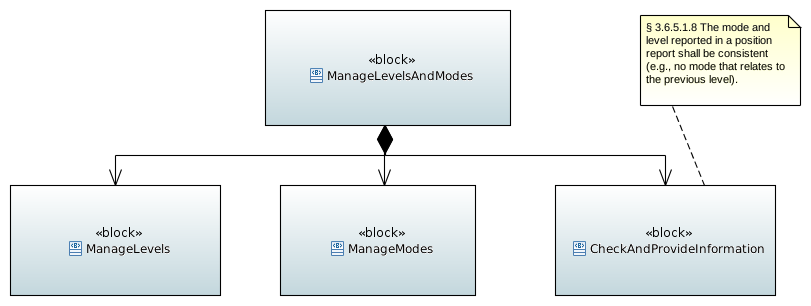
\includegraphics[scale=1]{../SysML/FunctionalArchitecture.png}
\caption{High level Architecture}
\end{figure}
\end{landscape}

This function is shared in three subfunctions: 
\begin{description}
\item[Manage modes] computes the new mode to apply according conditions from inputs and other functions (see \citep{subset-026} sections 4.4, 4.6, 5.4, 5.5, 5.6, 5.7, 5.8, 5.9, 5.11, 5.12, 5.13, 5.19)
\item[Manage levels] computes the new level to apply according inputs (see \citep{subset-026} section 5.10)
\item[Provide output] checks compatibility between mode and level and provides outputs (see \citep{subset-026} section 3.6.5)
\end{description}

\begin{landscape}
\begin{figure}[hbtp]
\centering
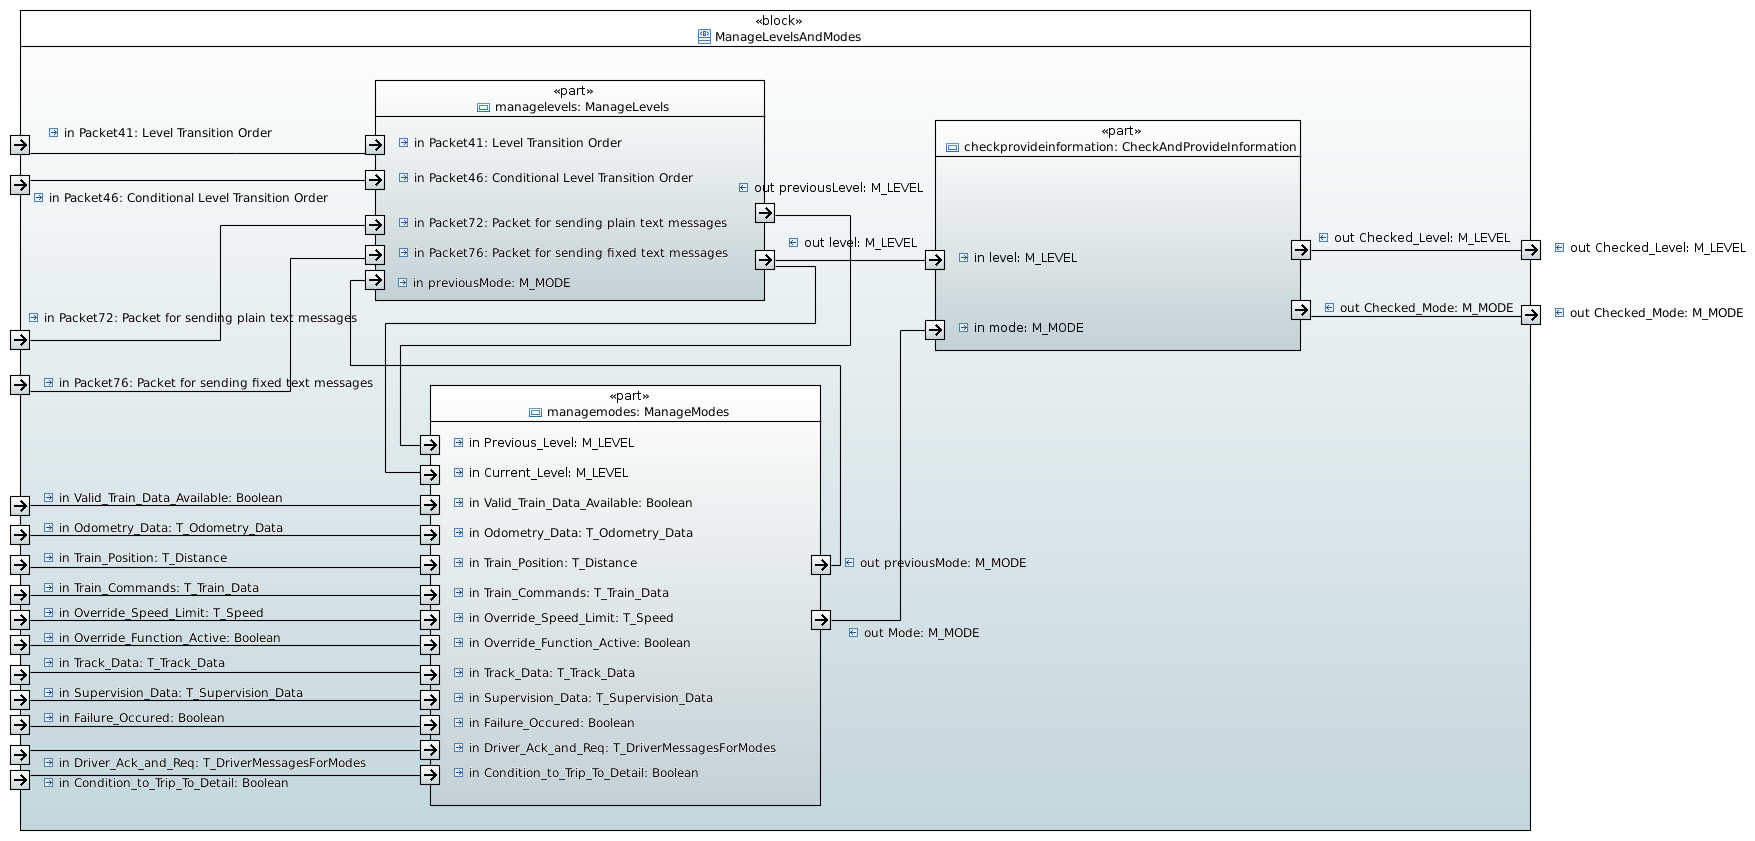
\includegraphics[scale=0.6]{../SysML/ManageLevelsAndModes.png}
\caption{High level dataFlow}
\end{figure}
\end{landscape}

The previous figure show the main interface of this function, according to the type defined as follow:

\begin{landscape}
\begin{figure}[hbtp]
\centering
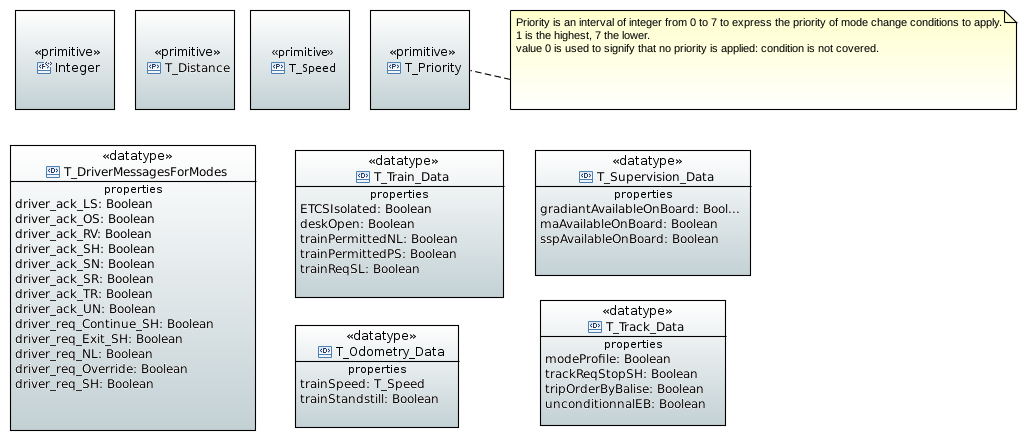
\includegraphics[scale=0.9]{../SysML/DataTypes.png}
\caption{Data Types}
\end{figure}
\end{landscape}

% end of chapter

\chapter{Modes}

% \chapter{Modes}

\section{Architecture - SysML}


This function is in charge of the computation of new mode to apply in fonction of conditions from inputs and other functions.

\begin{landscape}
\begin{figure}[hbtp]
\centering
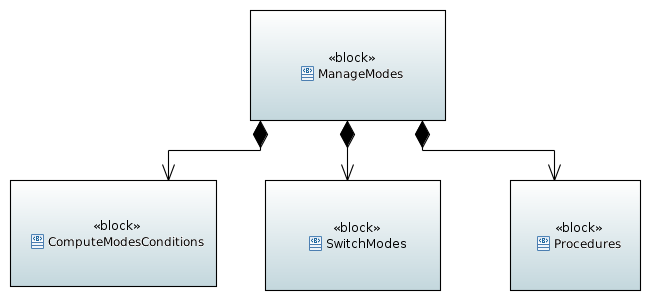
\includegraphics[scale=1]{../SysML/FunctionalArchi_Modes.png}
\caption{Modes subfubction architecture}
\end{figure}
\end{landscape}

Three subfunctions are defined:
\begin{description}
\item[ComputeCondition] specifies the conditions to define a mode transition according condition table of section 4.6.3 of \citep{subset-026}
\item[SwitchModes] performs the mode selection according the conditions and priorities defined in transition table  section 4.6.2 of \citep{subset-026}
\item[Procedures] performs all specific procedure linked to mode management and defined in  \citep{subset-026} sections 5.4, 5.5, 5.6, 5.7, 5.8, 5.9, 5.11, 5.12, 5.13, 5.19.
\end{description}


See below section "Detailled model" for details.

\begin{landscape}
\begin{figure}[hbtp]
\centering
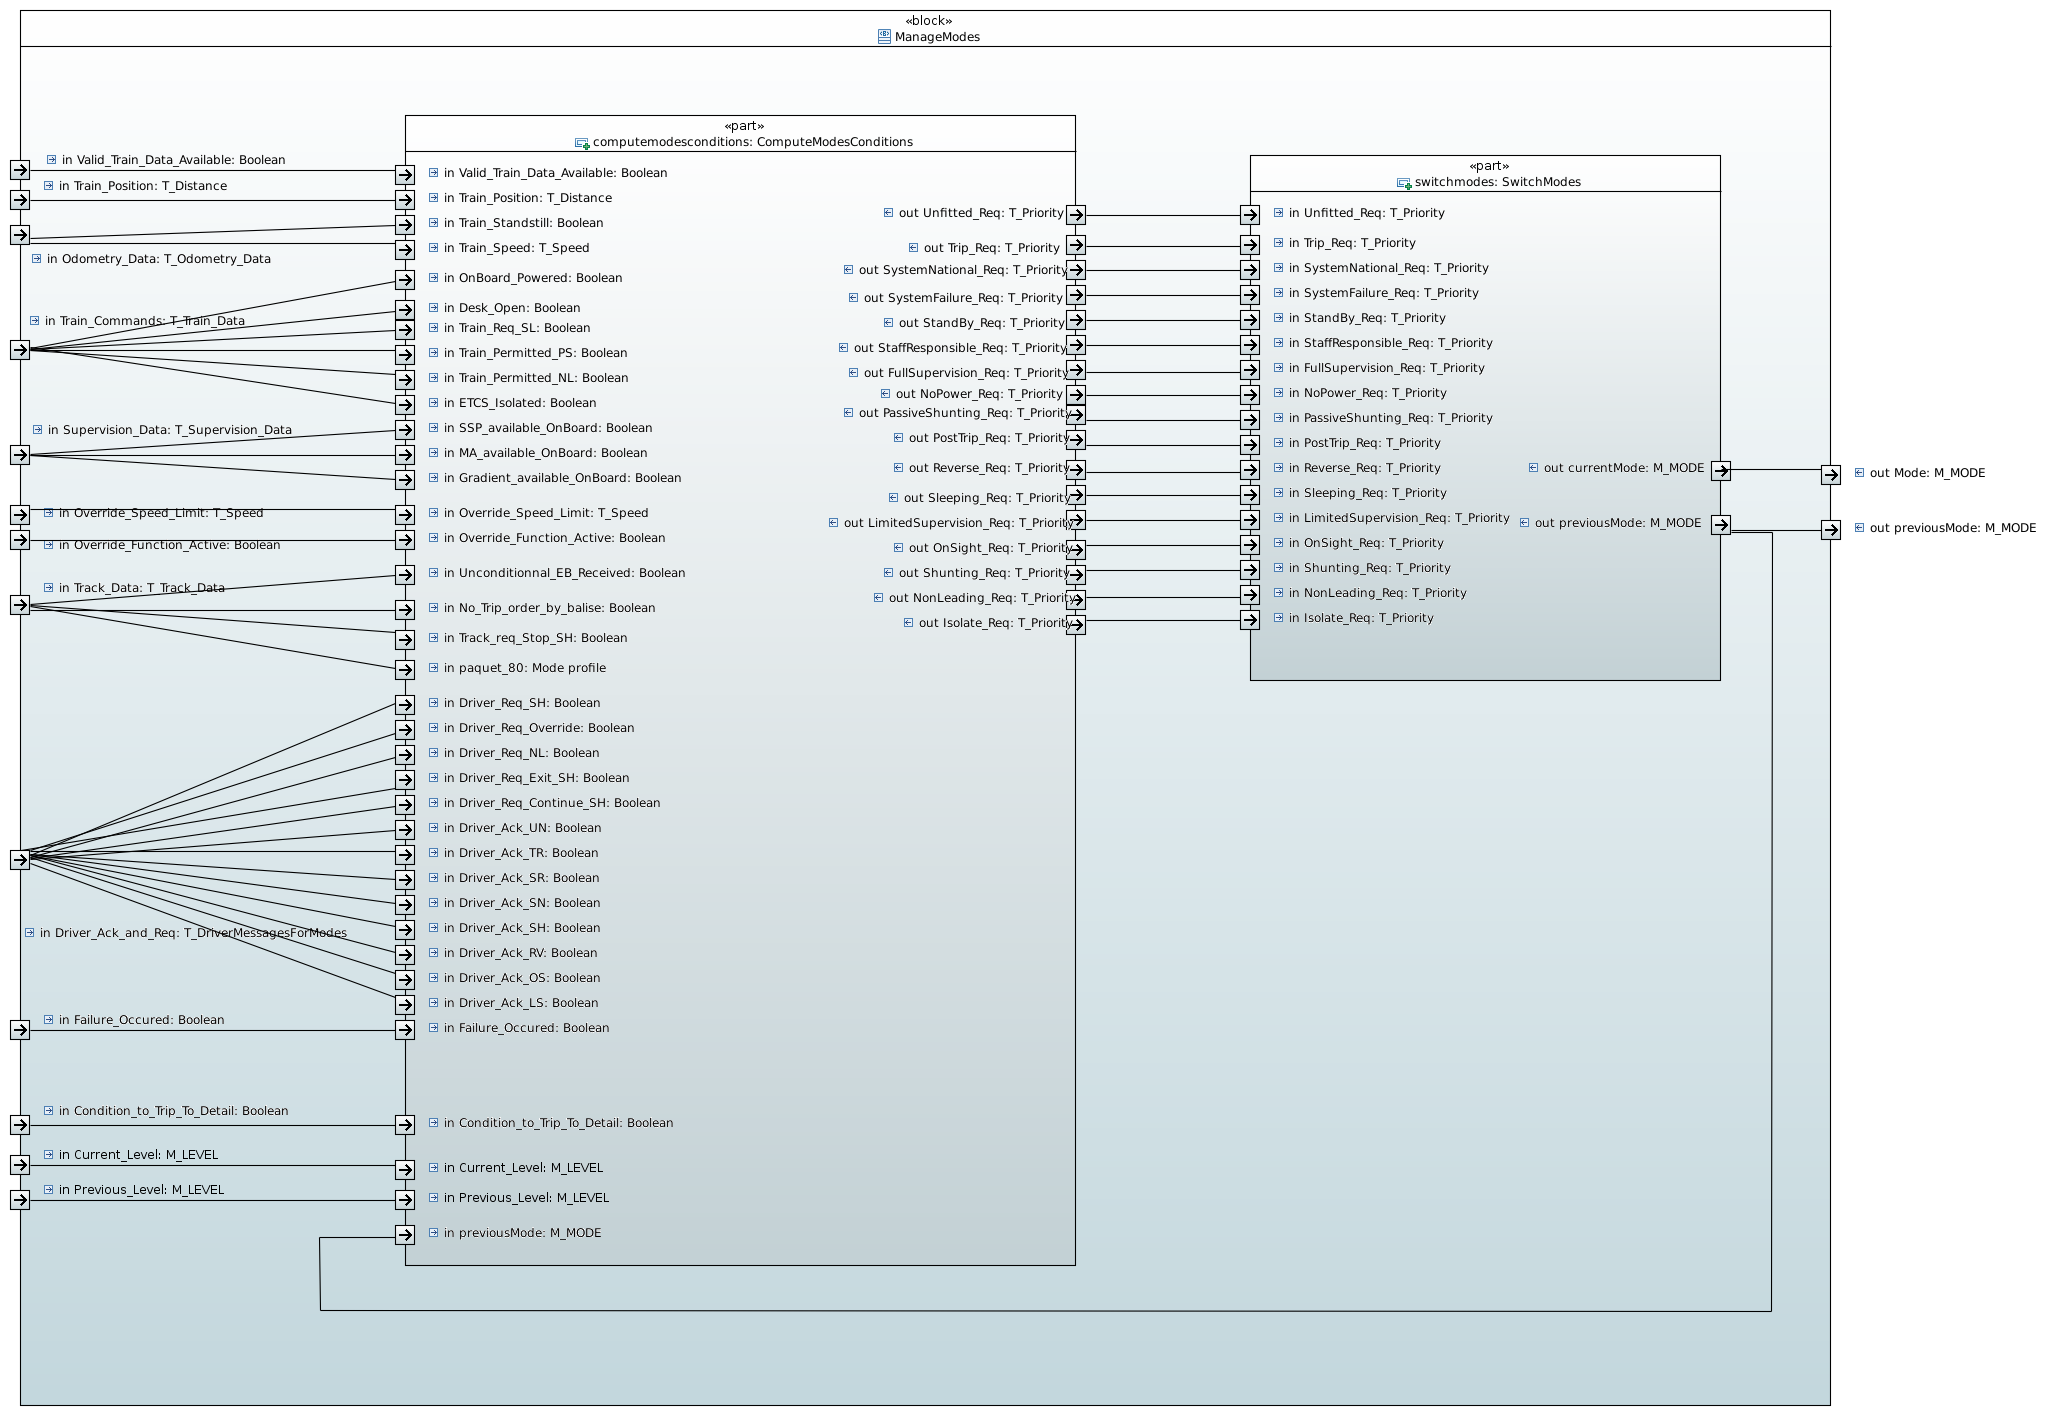
\includegraphics[scale=0.45]{../SysML/ManageModes.png}
\caption{Modes subfunction dataflow}
\end{figure}
\end{landscape}

\section{Interface}

\subsection{Public Types of Modes}


\begin{center}


\renewcommand{\arraystretch}{2} 
\tablehead{%
\hline
\rowcolor{gray} 
Name & Type &  Comments  \\ 
\hline}
\tablefirsthead{
\hline
\rowcolor{gray} 
Name & Type &  Comments  \\ 
\hline 
}
\begin{supertabular}{| m{3cm} | m{6cm} | m{4cm} |}
\hline 
T\_Cab	& enum \{A, B, unknown\}	& Assumption : Train has exactly two cabins see \citep{subset-034} \\ 
\hline
T\_Level & 	enum \{L0, L1, L2, L3, LNTC\}	& \textcolor{blue}{To check with level section}  \\ 
\hline
T\_Mode	& enum \{NP, SB, PS, SH, FS, LS, SR, OS, SL, NL, UN, TR, PT, SF, IS, SN, RV\}	& M\_MODE can not be used: No power mode is not defined. \\ 
\hline
T\_MA	& enum \{Profile\_OS, Profile\_LS, Profile\_SH, No\_Profile\}	& M\_MAMODE can not be used: No Profile is not defined. \\ 
\hline
T\_Mode\_Profile & 	Structure \{Distance : int, Mode :  T\_MA, Speed : int, Length : int, Length\_Ack : int \}	 & \textcolor{red}{To check with filtering function and internal structure.}  \\ 
\hline 
\end{supertabular} 


\end{center}

\subsection{Inputs of ManageModes}


\begin{center}

\tablehead{%
\hline
\rowcolor{gray} 
Name & Type & Consummers & Comments  \\ 
\hline}
\tablefirsthead{
\hline
\rowcolor{gray} 
Name & Type & Consummers & Comments  \\ 
\hline 
}
\begin{supertabular}{| m{6cm} | m{3cm} | m{3cm} | m{3cm} |}
\hline 
Ack\_Req\_LS\_Display  & bool & To Dmi & procedure ?  \\ 
\hline 
Ack\_Req\_OS\_Display  & bool & To Dmi & procedure ?  \\ 
\hline  
Ack\_Req\_SH\_Display  & bool & To Dmi & procedure ?  \\ 
\hline 
Ack\_Req\_SN\_Display & bool & To Dmi & procedure ?  \\ 
\hline 
Ack\_Req\_SR\_Display & bool & To Dmi & procedure ?  \\ 
\hline 
Ack\_Req\_UN\_Display & bool & To Dmi & procedure ?  \\ 
\hline 
Cab &	T\_Cab	& From TIU &  \\ 
\hline 
ConditionToTrip & bool & To clarify& • \\ 
\hline 
Continue\_Shunting\_Function\_Active & bool &  Procedure ?& • \\ 
\hline 
CurrenT\_Level	& T\_Level	& Internal from Level Management& • \\ 
\hline 
Desk\_A\_Open & bool & From TIU & • \\ 
\hline 
Desk\_B\_Open & bool & From TIU & • \\ 
\hline 
Driver\_Ack\_LS & bool & From DMI & procedure ?  \\ 
\hline 
Driver\_Ack\_OS & bool & From DMI & procedure ?  \\ 
\hline 
Driver\_Ack\_RV & bool & From DMI & procedure ?  \\ 
\hline 
Driver\_Ack\_SH & bool & From DMI & procedure ?  \\ 
\hline 
Driver\_Ack\_SN & bool & From DMI & procedure ?  \\ 
\hline 
Driver\_Ack\_SR & bool & From DMI & procedure ?  \\ 
\hline 
Driver\_Ack\_TR & bool & From DMI & procedure ?  \\ 
\hline 
Driver\_Ack\_UN & bool & From DMI & procedure ?  \\ 
\hline 
Driver\_Req\_ExiT\_SH & bool & From DMI & procedure ?  \\ 
\hline 
Driver\_Req\_NL & bool & From DMI & procedure ?  \\ 
\hline 
Driver\_Req\_Override & bool & From DMI & procedure ?  \\ 
\hline 
Driver\_Req\_SH & bool & From DMI & procedure ?  \\ 
\hline 
Emergency\_Stop\_Message\_Received & bool & From Balises ?& • \\ 
\hline 
Estimated\_Front & int & Train position ?& • \\ 
\hline 
ETCS\_Isolated & bool & From TIU& • \\ 
\hline 
Failure\_Occured & bool & Internal ?& • \\ 
\hline 
Previous\_Level & 	T\_Level	& Internal from Level Management& • \\ 
\hline 
MA\_SSP\_Gradiant\_Available & bool & From supervision ?& • \\ 
\hline 
Max\_Safe\_Front & bool & Train position ?& • \\ 
\hline 
Mode\_Profile\_On\_Board &	T\_Mode\_Profile &	Stored from  packet 80 & • \\ 
\hline 
No\_Trip\_Order\_Given\_By\_Balise & bool & From Balises ?& • \\ 
\hline 
OnBoard\_Powered & bool & From TIU& • \\ 
\hline 
Override\_Function\_Active & bool & Procedure ?& • \\ 
\hline 
Shunting\_Granted\_By\_RBC & bool & Radio ?& • \\ 
\hline 
Stop\_Shunting\_Stored & bool & Procedure ?& • \\ 
\hline 
Train\_Permitted\_NL & bool & From TIU& • \\ 
\hline 
Train\_Permitted\_PS & bool & From TIU & • \\ 
\hline 
Train\_Req\_SL & bool & From TIU& • \\ 
\hline 
Train\_Speed\_Under\_Override\_Limit & bool & From supervision ?& • \\ 
\hline 
Train\_Standstill & bool & From supervision ?& • \\ 
\hline 
Train\_Speed & int & From supervision ?& • \\ 
\hline 
Valid\_Train\_Data\_Stored & bool & Internal ?& • \\ 
\hline 
\end{supertabular} 

\end{center}

\subsection{Outputs of ManageModes}

\begin{center}

\tablehead{%
\hline
\rowcolor{gray} 
Name & Type & Consummers & Comments  \\ 
\hline}
\tablefirsthead{
\hline
\rowcolor{gray} 
Name & Type & Consummers & Comments  \\ 
\hline 
}
\begin{supertabular}{| m{6cm} | m{3cm} | m{3cm} | m{3cm} |}
\hline 
currentMode & T\_Mode & • & • \\ 
\hline 
previousMode & T\_Mode & • & • \\ 
\hline 
\end{supertabular} 
	


\end{center}


\section{Requirements}

\section{Detailled model - SCADE}

\subsection{ComputeModesConditions subfunction}

\subsection{SwitchModes subfunction}


\subsection{Procedures subfunction}

% end of chapter


\chapter{Levels}

%\chapter{Levels}

\section{Architecture - SysML}


\begin{landscape}

\begin{figure}[hbtp]
\centering
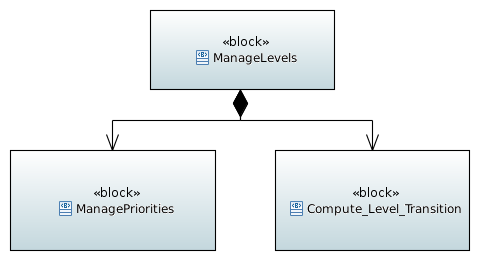
\includegraphics[scale=1]{../SysML/FunctionalArchi_Levels.png}
\caption{Levels subfunction architecture}
\end{figure}
\end{landscape}


\begin{landscape}
\begin{figure}[hbtp]
\centering
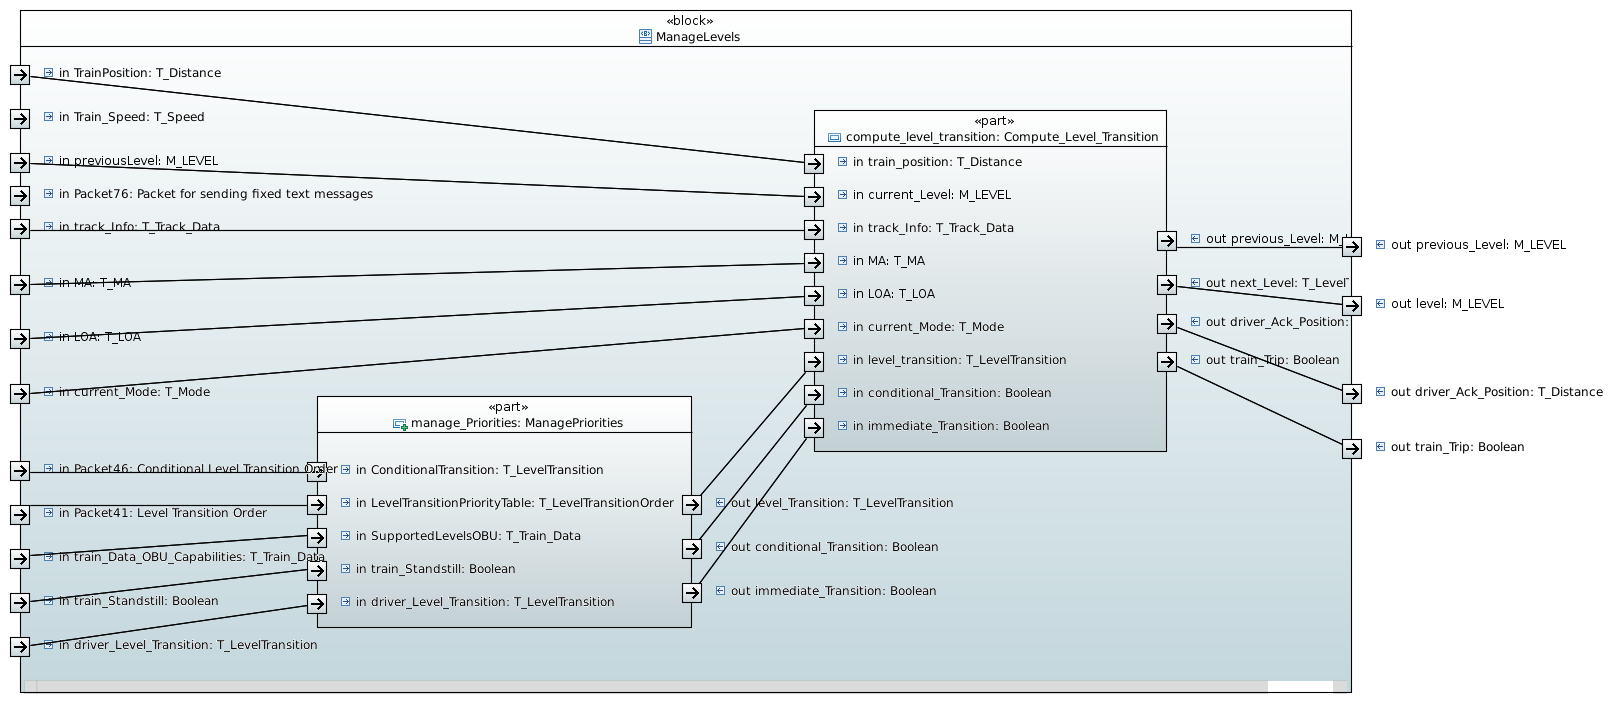
\includegraphics[scale=0.6]{../SysML/ManageLevels.png}
\caption{Levels subfunction dataflow}
\end{figure}
\end{landscape}

\section{Interface}

\section{Requirements}

\section{Detailled model - SCADE}


% end of chapter

\chapter{Provides}

% \chapter{Provides}

\section{Architecture - SysML}


\begin{landscape}
\begin{figure}[hbtp]
\centering
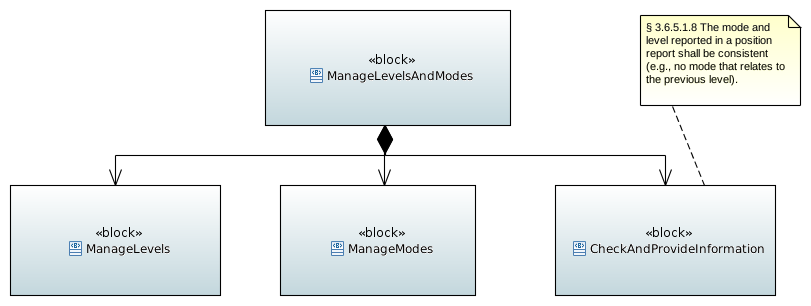
\includegraphics[scale=1]{../SysML/FunctionalArchitecture.png}
\caption{Provide subfunction Architecture}
\end{figure}
\end{landscape}


\section{Interface}

\section{Requirements}

\section{Detailled model - SCADE}

% end of chapter



\bibliographystyle{unsrt}
\bibliography{architecture}



\newpage
\addcontentsline{toc}{chapter}{Index}
\printindex
%===================================================
%Do NOT change anything below this line

\end{document}
